\documentclass[border=10pt]{standalone}

\usepackage{tikz}
\usepackage{tikzsymbols}
\usetikzlibrary{calc,patterns,shapes.geometric}

\def\centerarc[#1](#2)(#3:#4:#5){\draw[#1] ($(#2)+({#5*cos(#3)},{#5*sin(#3)})$) arc (#3:#4:#5);}

\begin{document}
	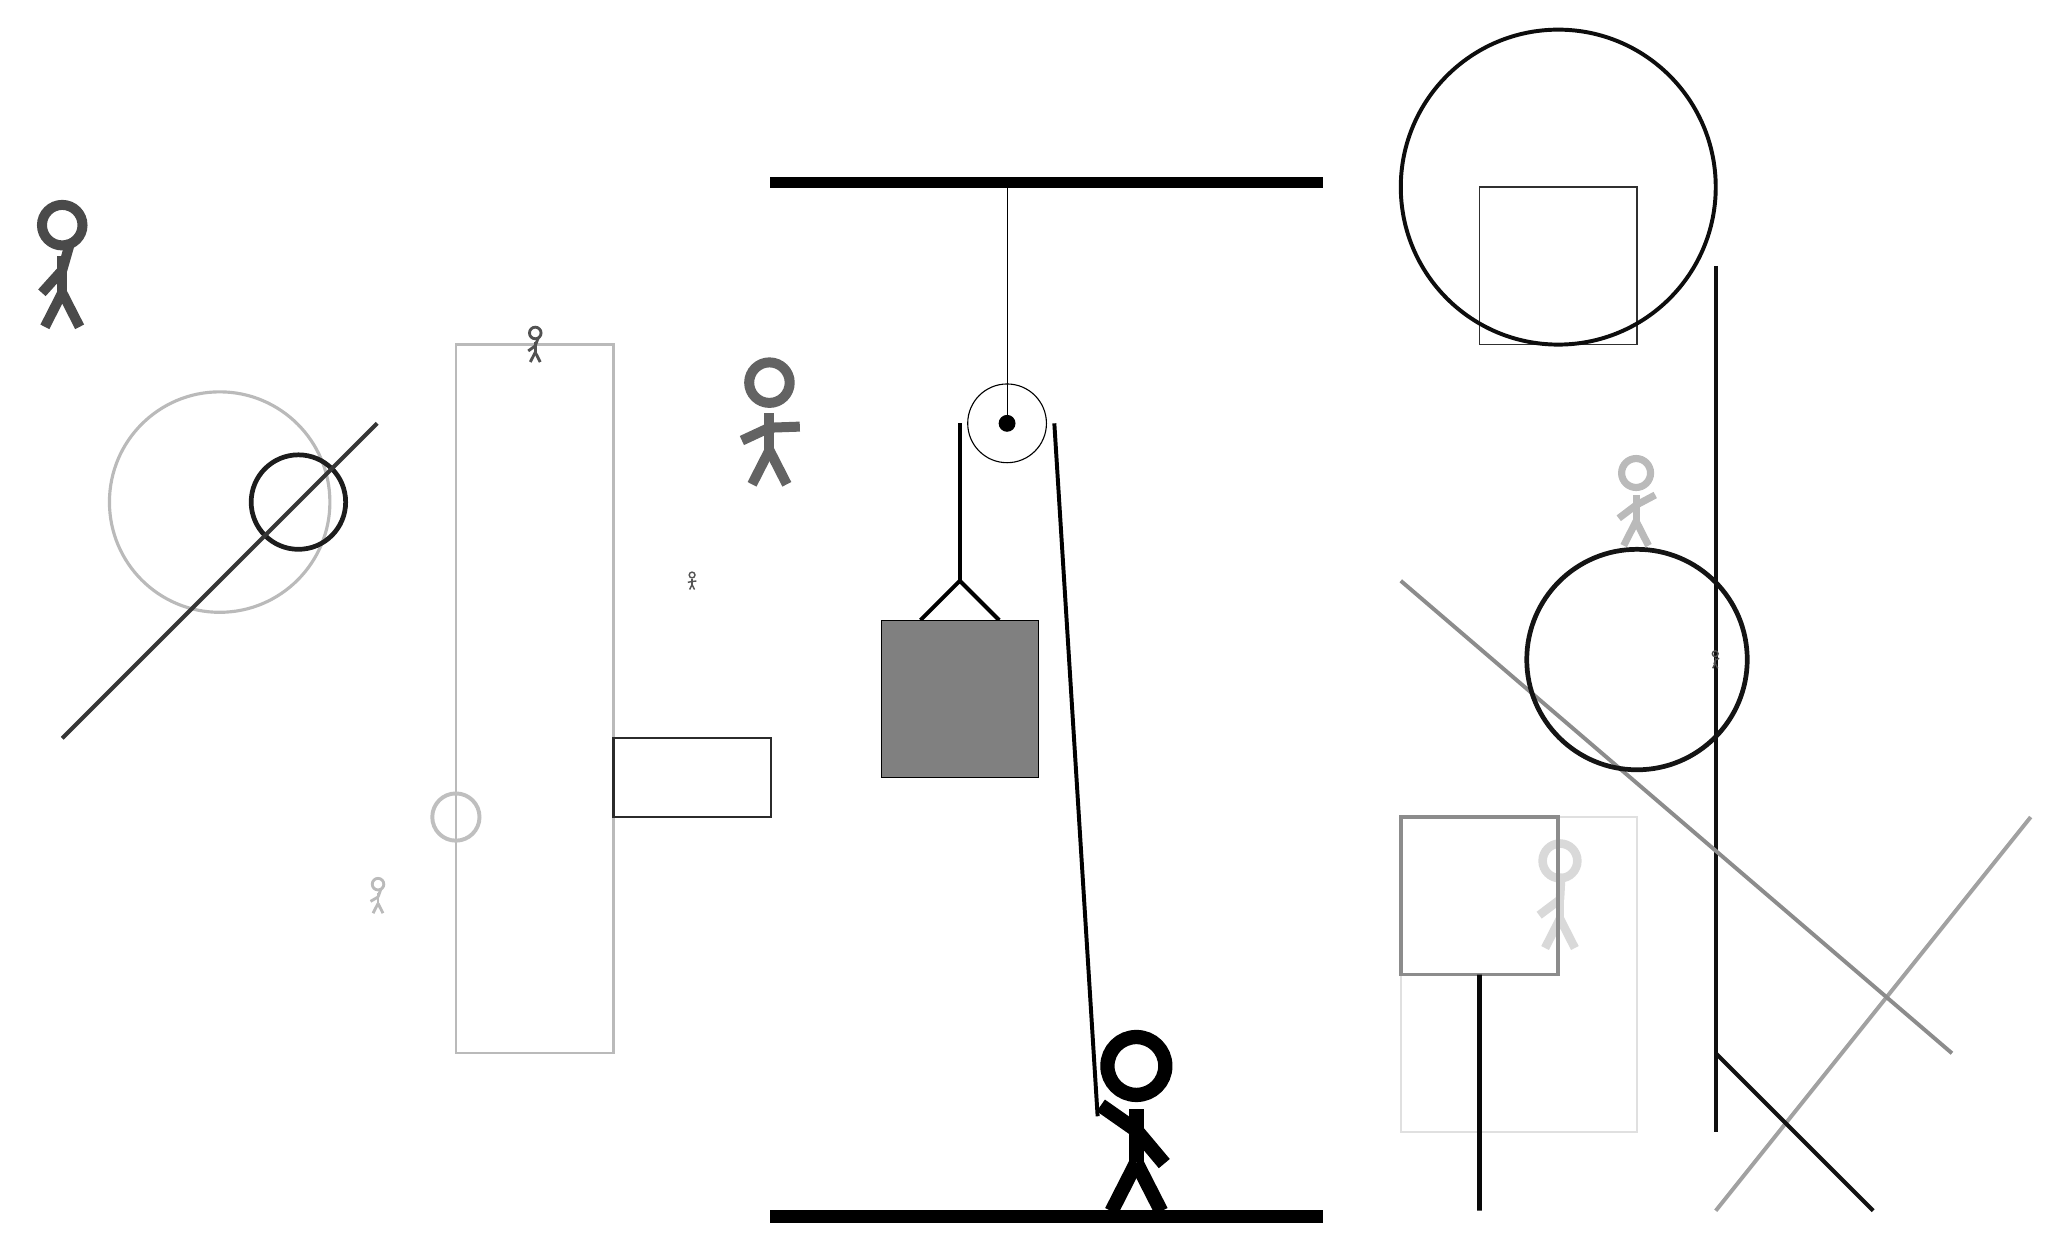
\begin{tikzpicture}
		%%%%% START %%%%%
		
		\draw[fill=black] (-2, 10) rectangle (5, 10.125);
		
		\draw (1, 7) circle (0.5);
		\draw[fill=black] (1, 7) circle (0.1);
		\draw (1, 10) -- (1, 7);
		
		\draw[line width=0.5mm] (-0.1, 4.5) -- (0.4, 5.0) -- (0.9, 4.5);
		\draw[fill=black!50] (-0.6, 4.5) rectangle (1.4, 2.5);
		
		\draw[line width=0.2mm, color=black!12] (6, -2) rectangle (9, 2);
		
		\node[line width=0.3mm, color=black!15] at (8, 1) {\Strichmaxerl[6][37][87]};
		\draw[line width=0.5mm, color=black!94](10, 9) -- (10, -2);
		\draw[line width=0.2mm, color=black!81] (7, 8) rectangle (9, 10);
		
		\draw[line width=0.3mm, color=black!27] (-4, -1) rectangle (-6, 8);
		
		\draw[line width=0.5mm, color=black!37](10, -3) -- (14, 2);
		\draw[line width=0.5mm, color=black!45](6, 5) -- (13, -1);
		\draw[line width=0.5mm, color=black!45] (6, 0) rectangle (8, 2);
		\draw [line width=0.5mm, color=black!25](-6, 2) circle (0.3);
		
		\draw[line width=0.3mm, color=black!83] (-2, 2) rectangle (-4, 3);
		\draw [line width=0.4mm, color=black!27](-9, 6) circle (1.4);
		\node[line width=0.6mm, color=black!27] at (-7, 1) {\Strichmaxerl[2][30][70]};
		\draw [line width=0.6mm, color=black!92](9, 4) circle (1.4);
		
		\draw[line width=0.7mm, color=black!97] (7, -3) rectangle (7, 0);
		\node[line width=0.4mm, color=black!67] at (-3, 5) {\Strichmaxerl[1][12][5]};
		\draw [line width=0.6mm, color=black!89](-8, 6) circle (0.6);
		
		\node[line width=0.6mm, color=black!70] at (10, 4) {\Strichmaxerl[1][73][26]};
		
		\node[line width=0.7mm, color=black!68] at (-5, 8) {\Strichmaxerl[2][36][70]};
		\draw [line width=0.5mm, color=black!95](8, 10) circle (2.0);
		\draw[line width=0.5mm, color=black!93](10, -1) -- (12, -3);
		\node[line width=0.2mm, color=black!27] at (9, 6) {\Strichmaxerl[5][37][28]};
		
		\node[line width=0.2mm, color=black!61] at (-2, 7) {\Strichmaxerl[7][25][2]};
		\draw[line width=0.5mm, color=black!79](-7, 7) -- (-11, 3);
		\node[line width=0.5mm, color=black!71] at (-11, 9) {\Strichmaxerl[7][48][74]};
		
		\draw[line width=0.5mm] (0.4, 7) -- (0.4, 5.0);
		\centerarc[line width=0.5mm](1, 7)(0:180:0.6);
		\draw[line width=0.5mm](1.6, 7) -- (2.15, -1.8);
		
		\node at (2.6, -1.9) {\Strichmaxerl[10][-35][-50]};
		
		\draw[fill=black] (-2, -3) rectangle (5, -3.15);
		
		%%%%% END %%%%%
	\end{tikzpicture}
\end{document}